%======================================================================
\chapter{Model Implementation}
%======================================================================
\section{Introduction}

This chapter discusses the methodology of calculating the warpage and the residual stress in the wafers cut via wire sawing from directionally solidified ingots. The methodology comprises of the ABAQUS implementation of the model developed in the previous chapter using the governing equations discussed in the literature review. 

%This chapter discusses the methodology of calculating the warpage and the residual stress in the wafers cut via wire sawing from directionally solidified ingots. The methodology comprises of the governing equations for directional solidification \& wire sawing and the model development. The governing equations have discussed in the literature review and the model development has been discussed in the previous chapter.   

%In this chapter, the finite element implementation of the model developed in the previous chapter is discussed using the governing equations discussed in the literature review section. 

As described in the literature review, several models have been built for simulating residual stress and dislocation density while the DS process of mc-Si ingots using dislocation creep behaviour of silicon. HAS creep model is used in this work to predict the dislocation density developed in silicon under stress. Analytical models for temperature change and material removal rate during wire sawing developed , respectively, by Bhagavat and Moller is used in developing the finite element simulation of wire sawing. The current work consists of three steps: first, simulation of directional solidification, second, mapping the results from above simulation on wire sawing mesh, third, simulation of wire sawing. The mapping was a challenging task since the directional solidification and wire sawing simulation were done on dissimilar meshes. 

The finite element models developed for thermal and simulation for directional solidification and wire sawing are same in terms of governing equations. However, they differ in the initial and boundary conditions along with the meshing and step formulations. While the sequentially coupled thermal-stress simulation of directional solidification is straight forward, the mapping stage and the wire sawing simulation is sophisticated. So their details have been discussed in the later sections.

\section{Governing equations}
The overall strain in a system is the summation of strain contributions from several factors. In the current work, total strain is assumed to be the sum of elastic, plastic, thermal and dislocation creep strain


\begin{equation}
\epsilon_{s} = e^{el} + e^{pl} + e^{thermal} +e^{creep}
\label {strainEq2}
\end{equation}



\begin{comment}

In matrix form, the linear elastic strain for an isotropic material can be written 

\begin{equation} 
\begin{Bmatrix}
 \epsilon_{11}   \\ 
 \epsilon_{22}   \\
 \epsilon_{33}   \\
 \gamma_{12}   \\
 \gamma_{13}   \\
 \gamma_{23}
\end{Bmatrix} = \begin{bmatrix}
 1/E & -v/E & -v/E &  0 &  0 &  0  \\ 
 -v/E & 1/E & -v/E & 0 & 0 & 0  \\ 
 -v/E & -v/E & 1/E &  0 &  0 &  0  \\ 
 0 & 0 & 0 & 1/G & 0 &  0  \\ 
 0 & 0 & 0 & 0 & 1/G & 0  \\ 
 0 & 0 & 0 & 0 & 0 & 1/G  
\end{bmatrix} \begin{Bmatrix}
 \sigma_{11}   \\ 
 \sigma_{22}   \\
 \sigma_{33}   \\
 \sigma_{12}   \\
 \sigma_{13}   \\
 \sigma_{23}
\end{Bmatrix}

\label {strain_matrix}
\end{equation}
\end{comment}

Solving any time varying stress-strain constitutive relation requires knowledge of time varying strain. Time varying linear elastic strain is thus given by
\begin{equation} 
\dot{\epsilon}^{e}_{s} = \frac{1+v}{E}\dot{\sigma}_{s} 
                        - \frac{v}{E}tr(\dot{\sigma}_{s})I
\label {hyperelasticEq}
\end{equation}

Similarly, time varying thermal strain is given by
\[ \dot{\epsilon}^{T}_{s} = \alpha \dot{T} I \] 
In this simulation, yielding and subsequent plastic deformation is not considered. So the plastic strain rate is considered 0
\[ \dot{\epsilon}^{p}_{s} = 0 \]

HAS model was used to calculate the dislocation creep strain rate. As discussed in literature review, HAS model related the creep strain rate with the dislocation density. In the multiaxial form HAS equation can be written as
\begin{equation} 
\dot{\epsilon}^{creep}_{s} = \frac{1}{2} b k_{0} (\tau_{eff})^{P} exp(-Q/k_{b}T) N_{m}
\frac{1}{\sqrt{J_{2}}} \cdot S_{ij}
\label {HAS_Eq}
\end{equation}
 
\[ \dot{N}_{m} = K k_{0} (\tau_{eff})^{P+\lambda} exp(-Q/k_{b}T) N_{m}  \] 
  
 
\[ J_{2} = 1/S_{ij}S_{ij} \]

\[ S_{ij} = \sigma_{ij} -1/3\sigma_{kk} \delta_{ij} \]

Where $b$ is the magnitude of the Burgers vector, $\tau_{eff}$ the effective shear stress, $Q$ the Peierls potential, $k_{b}$ the Boltzman constant, $T$ the absolute temperature of the silicon crystal, $N_{m}$ the density of mobile dislocation at any time, $S_{ij}$ the deviator component of stress, $J_{2}$ the second invariant of the stress deviator, $D$ the strain hardening factor and $k_{0}$, $K$, $p$ and $\lambda$ the material constants. $\tau_{eff}$ is written as

\begin{equation}
   \tau_{eff} = \tau -  D\sqrt{N_{m}} \label{tau_eff2}
\end{equation}

\begin{comment}

Mass continuity equation inside the domain of ingot can be written as

\[ \triangledown \cdot \sigma = 0 \]

In case of a cylindrical geometry the partial differential equations for above equation can be written as

\[ \frac{1}{r}\frac{\partial}{\partial r} (r \sigma_{rr})
+ \frac{\partial}{\partial z} \sigma_{rz} - \frac{\sigma_{\theta \theta}}{r} + b_{r} = 0
\]
\[ \frac{1}{r}\frac{\partial}{\partial r} (r \sigma_{zr})
+ \frac{\partial}{\partial z} \sigma_{zz} + b_{z} = 0\]

\[ \epsilon_{rr} = \frac{\partial u_{r}}{\partial r},\quad
                    \epsilon_{zz} = \frac{\partial u_{z}}{\partial z}, \quad
                    \epsilon_{\theta \theta} = \frac{u_{r}}{r}, \quad
                    \gamma_{rz} = \frac{\partial u_{r}}{\partial z} 
                    + \frac{\partial u_{z}}{\partial r} 
                    = \epsilon_{rz} + \epsilon_{zr}
                    = 2\epsilon_{rz}

\]

Where sigma-rr, sigma-zz, sigma-00 and sigma-rz are the normal stresses in the radial, axial, and azimuthal directions and the shear stress respectively. Due to presence of a radial symmetry of temperature distribution inside the ingot during solidification, the stress and the strain fields will be also be axisymmetric. This means that U-THETA and DEL/DEL-THETA terms will be 0. The equilibrium and the strain-displacement equations can be re written as 
\end{comment}


The stress relaxation is obtained through Hooke's law with substituting the value of elastic strain with total, thermal and creep strain
\begin{equation}
[\sigma] = [D^{el}] [\epsilon^{el}] 
\end{equation}

\[ [\epsilon^{el}] = [\epsilon - \epsilon^{thermal} - \epsilon^{creep}]\]


The stiffness matrix $[D^{el}]$ depends upon the Young's modulus and the Poisson's ratio, whose value are provided as material properties during the analysis

\section{Wire Sawing}
Finite element model of wire sawing was developed to simulate the material removal due to wire movement along the cutting direction. This was done by discretizing the material removal process into several small steps. During each of these steps, one row elements were removed from the mesh to simulate the thin layer of material removed. The heat that enters into the work piece is supplied as heat flux at each of these steps. The magnitude of this heat flux is as per discussed in SECTION X.X. On removal of material, new surface is created through which surface convection starts. To simulate this, surface convection property was activated on the surface created by the removal of element. 
The time duration for the steps were not uniform. Although the overall simulation was done for a 400 minute wire sawing process, time size $\triangle t^{i}$ for all the steps $i=1,2,..$ were not equal. This is because, as discussed in SECTION X.X, the material removal rate $v_{s}$ at depth of cut $x$ depends on the wire-material contact length $L_{x}$. 

\begin{equation}
v_{s} =  \frac{1}{\alpha  L_{x} \ }
\label {cr-slip4}
\end{equation}

The time step size $\triangle t_{x}^{i}$ required  to remove a strip of material $\triangle x^{i}$ at depth of cut $x$ at the $i$th step can be written as

\[ \triangle t_{x}^{i} = \frac{\triangle x^{i}}{v_{s}^{i}}  \]

\begin{equation}
\triangle t_{x}^{i} = \alpha L_{x}^{i} \triangle x^{i}
\label {time-step}
\end{equation}

\[ L_{x} = 2 \sqrt{R^{2}-(R-x)^{2})} \]

where $\alpha$ is a parameter than depends on slurry, abrasives and other things and its constant at all steps and $R$ is the work piece radius. The value of $\alpha$ is approximated in this work based on the total time the wire sawing process takes. Total time can be written as integration of all the $\triangle t_{x}^{i}$

\[ \int_{0}^{T} dt = 2 \int_{-R}^{R} \alpha \sqrt{(R^{2}-(R-x)^{2})}dx \]

Since $\alpha$ is constant with $x$, it can be written that

\[ T = 2\alpha \int_{-R}^{R} \sqrt{(R^{2}-(R-X)^{2})}dx = 4\alpha R \]

\[ \alpha = 400/4R = 400/(4*125) = 0.8 \]

This value of $\alpha$ was used in Equation \ref{time-step} while discretizing the time steps for finite element formulation. This is however, a very loose approximation made to perform this simulation and may not be the best approach. 


\section{Mapping}

Since the casting simulations were done on a 2D axisymmetric mesh to save computational time, the next part was converting these axisymmetric results into 3D and then mapping them onto a mesh specifically developed for simulating wire sawing. This mapping of stress fields was a 3 step procedure, as shown in Figure \ref{fig:mappings}. First, the rotation of axisymmetric result, second, mapping this result on a different mesh occupying same volume, and third, deactivating the elements of the mesh where wire sawing simulation is not being done.

\noindent
\begin{minipage}[c]{\textwidth}
\centering
        \captionsetup{type=figure}
        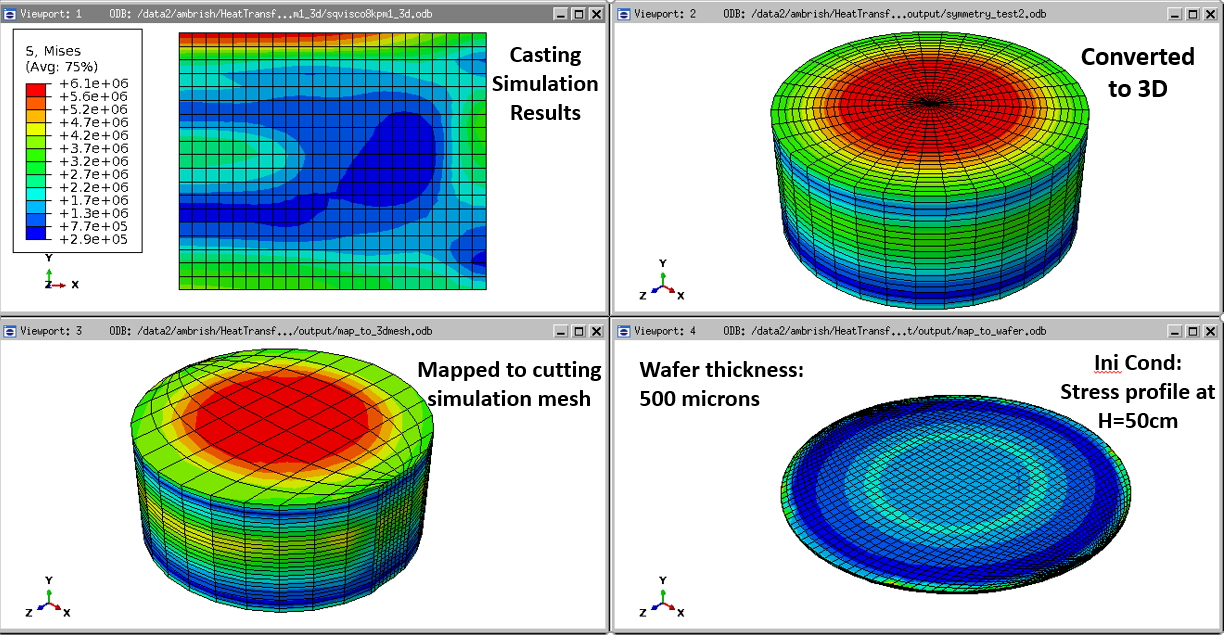
\includegraphics[width=6.0in]{mappings.PNG}
        \captionof{figure}{}.
        \label{fig:mappings}
 \end{minipage}


\begin{minipage}[c]{\textwidth}
\centering
        \captionsetup{type=figure}
        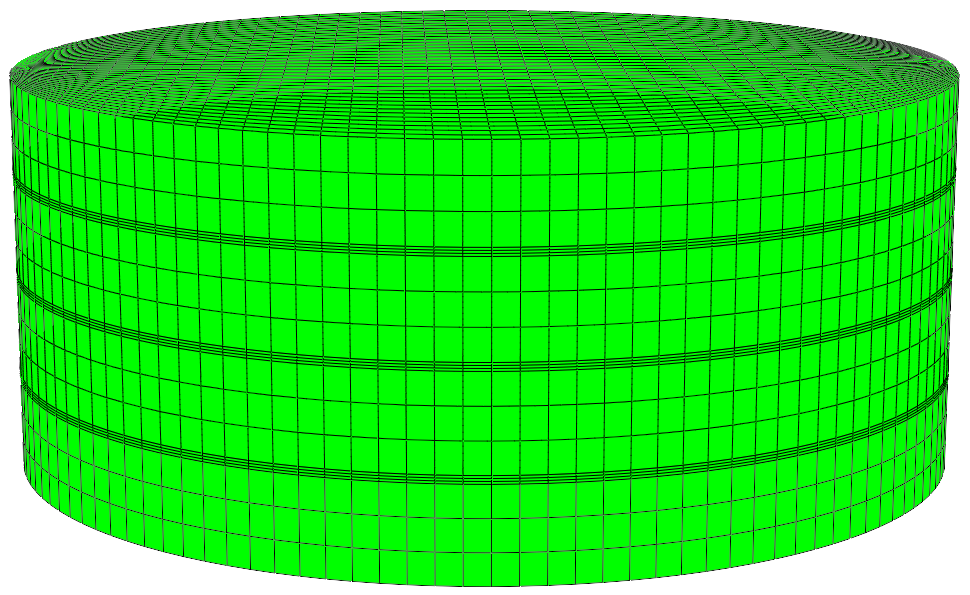
\includegraphics[width=2.0in]{wire-saw-mesh.PNG}
        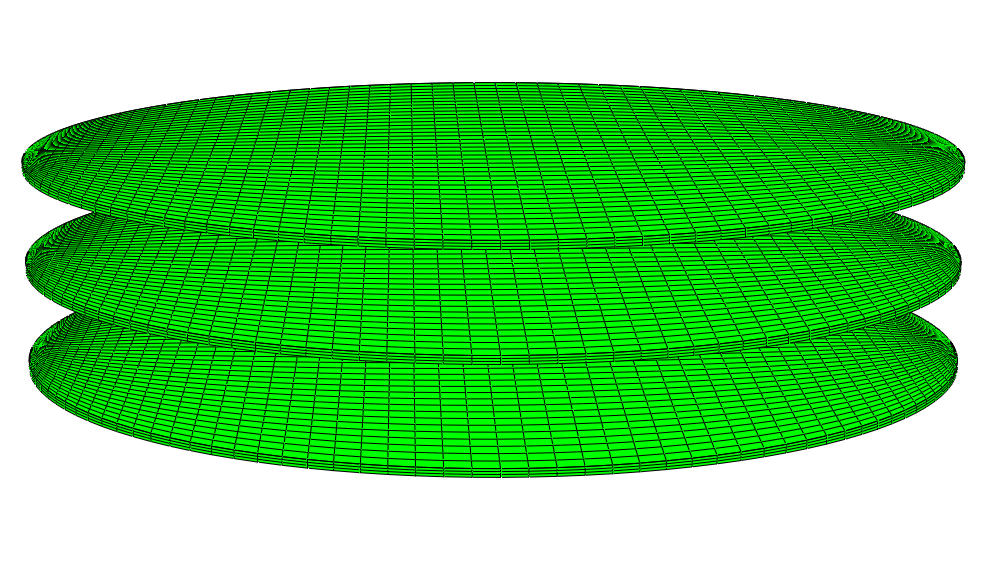
\includegraphics[width=2.0in]{wafer-kerf2.PNG}
        \captionof{figure}{}.
        \label{fig:model_change}
 \end{minipage}

%The volume where wire sawing simulation was done was 1000 micron thick sections at heights: 26.25,  52.5 & 79.75 mm, as shown in Figure \ref{fig:model_change}. These sections were 1000 micron thick because the wafer formed and the layers removed are both 500 micron as shown in Fig \ref{fig:cutting}. 

\begin{minipage}[c]{\textwidth}
\centering
         \captionsetup{type=figure}
        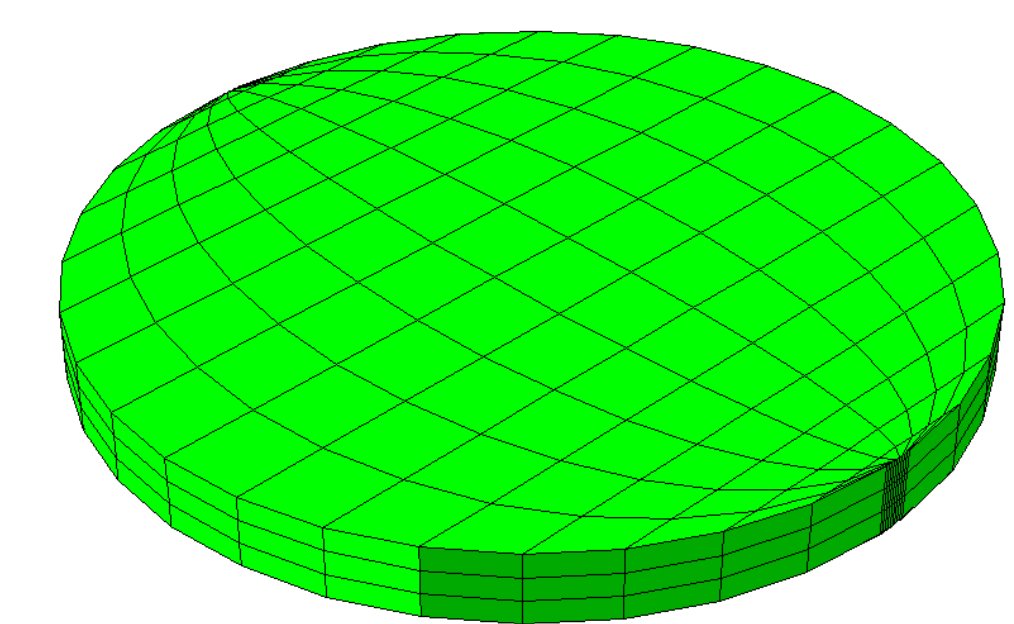
\includegraphics[width=2.0in]{cutting1.PNG}
        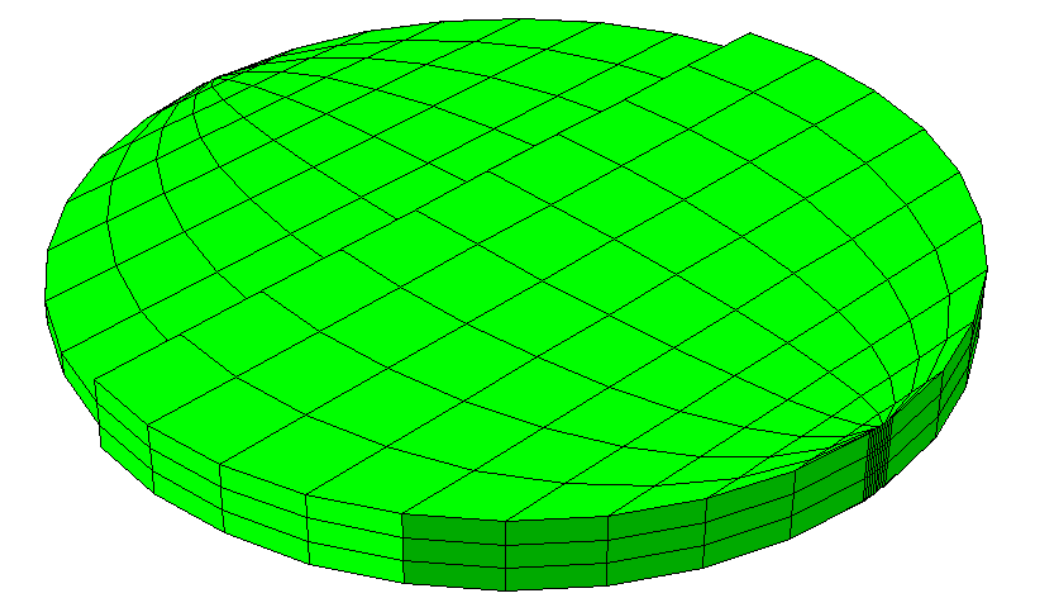
\includegraphics[width=2.0in]{cutting2.PNG}
        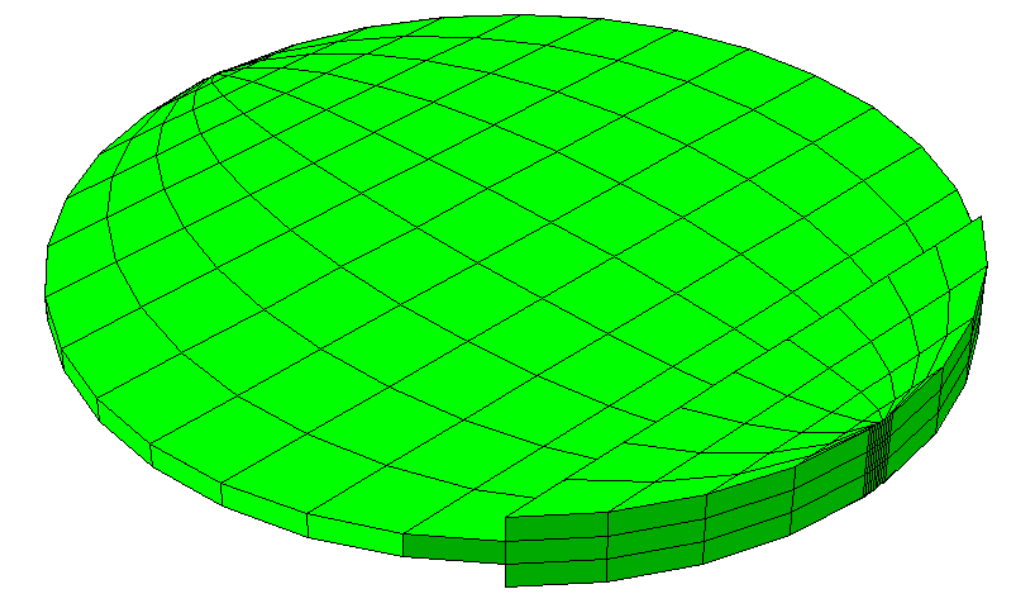
\includegraphics[width=2.0in]{cutting3.PNG}
        \captionof{figure}{}.
        \label{fig:cutting}
 \end{minipage}


